\section{Tipo de algoritmos de Machine Learning}
\label{sec:ml-types}

Existem 4 tipos de algoritmos de aprendizagemm, são eles \textbf{Aprendizagem supervisionada}, \textbf{Aprendizagem não-supervisionada},
\textbf{Aprendizagem semi-supervisionada} e \textbf{Aprendizagem por reforço}, extimasse que 70\ dos algoritmos de aprendizagem são de 
aprendizagem suprevisionada, e algo entre 20 a 10\ são não-supervisionada, enquanto o restante são os menos utilizados.

\subsection{Aprendizagem Supervisionada}
\label{subsec:supervised-learning}
Este tipo de algoritmo é utilizado quando a informação a ser utilizada para predição esta presente nos dados de treino, chamados de 
exemplos rotulados. Por exemplo um conjunto de dados de transações que possui um attributo que diz se é uma transação fraudulenta, o 
algoritmo procurará um padrão destes marcados como fraudulentos e gerará um modelo que indique a probabilidade de uma nova transação 
ser fraudulenta.

Aprendizagem supervisionada é mais apropriada e mais usada em aplicações que utilizão dados historicos para realizar predições. 
Basicamente utiliza-se padrões de dados rotulados para predizer novos dados não rotulados. 
Os métodos mais utilizados são \textbf{classificação}, \textbf{regressão} ou \textbf{predição numérica}.

O principal objetivo da aprendizagem supervisionada é construi um classificador que possa identificar a classe de novos dados apartir
do treinamento em exemplos rotulados.     


\subsubsection{Classicação}
\label{subsubsec:classificacao}

Classicação é um método que tem como objetivo categorizar novos dados em classes baseadas em atributos discretos ou qualitativo,
por exemplo um atributo é discreto quando assume um valor numérico de um conjunto finito de número ou uma quantidade enquanto que um
atributo qualitativo representa uma categoria como o sexo de uma pessoa podendo assumir o valor masculino ou feminino.
Em suma os novos dados são categorizados com base nas classes dos dados de treinamento (exemplos rotulados). 
Mas para que se possa estimar qual a classe destes novos dados é preciso de um \textbf{classificador},
este é o produto de um \textbf{indutor}, o objetivo de um indutor é extrair o melhor classificador possivel de um dado 
conjunto de exemplos rotulados.
Um classificador é gerado após exemplos rotulados serem submetidos á um dado indutor, após a geração do classificador 
é necessário identificar a qualidade do mesmo, apartir de métricas pré-definidas até atingir resultados aceitáveis, após a aceitação do classificador 
serão submetidos exemplos não rotulados e o classificador deverá enquadrar os dados em suas devidas classes com precisão. 
\begin{figure}[htb!]
	\centering
	\Caption{\label{fig:novo-classificador} Processo geração do classificador}	
	\UECEfig{}{
		\fbox{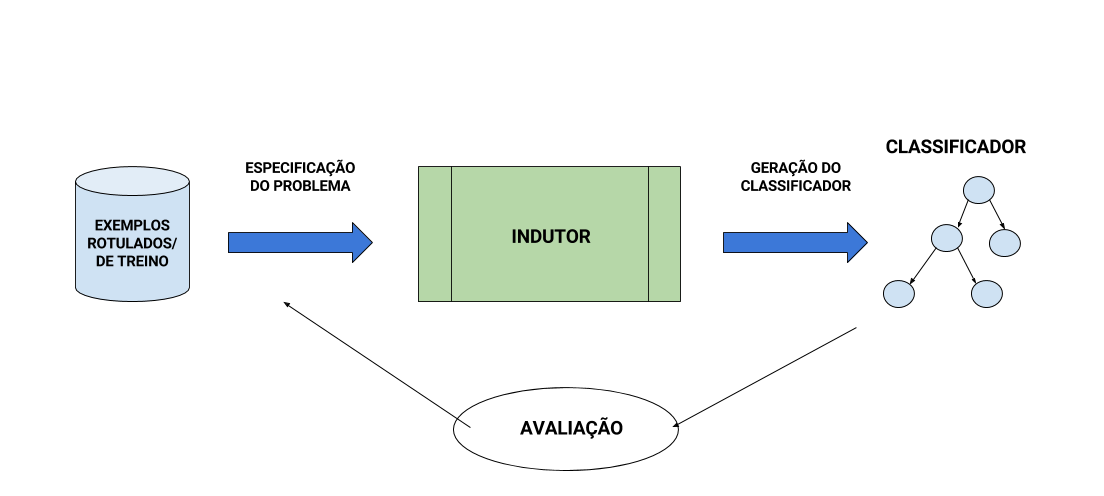
\includegraphics[width=14cm]{figuras/n-classifier}}
	}{
		\Fonte{Elaborado pelo autor}		
	}	
\end{figure}  

Ilustrando o exemplo de transações de cartão de crédito fraudulentas, dado que temos uma amostra de transações realizadas 
 Figura ~\ref{fig:amostra-transacoes}. Após estes dados serem submetidos ao classificador e irá predizar com um dado grau de probabilidade 
à qual classe o exemplo pertencem, logo sua saída basicamente será como aprensentado na Figura ~\ref{fig:amostra-transacoes-classefied}:
\begin{figure}[ht!]
	\centering
	\Caption{\label{fig:amostra-transacoes} Amostra de Transações de cartão de crédito}	
	\UECEfig{}{
		\fbox{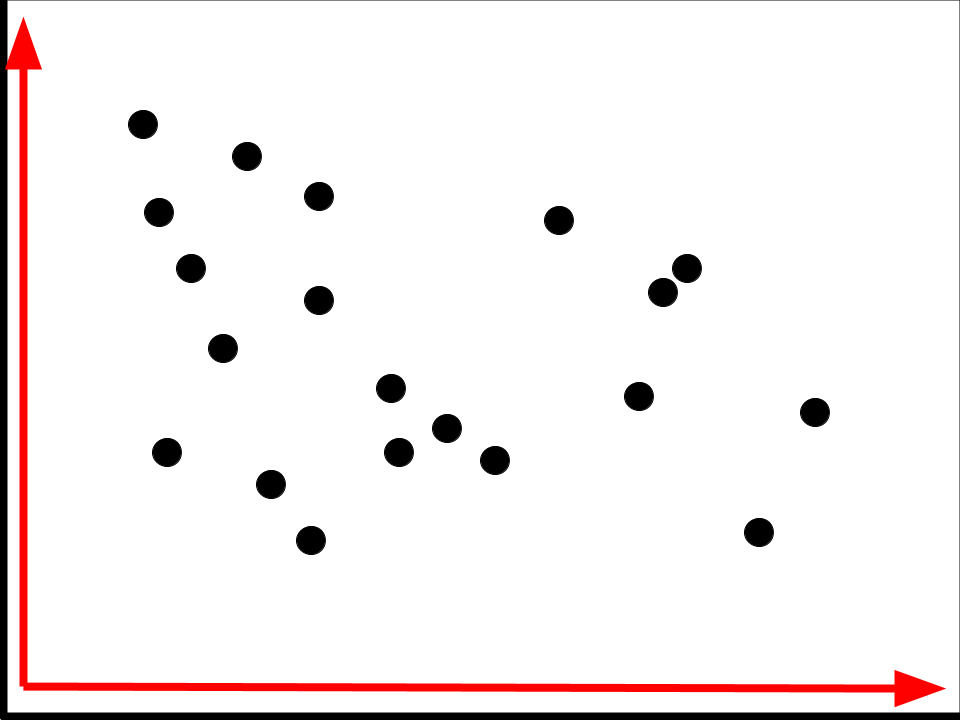
\includegraphics[width=8cm]{figuras/dados-nao-classificados}}
	}{
		\Fonte{Elaborado pelo autor}		
	}	
\end{figure}
\begin{figure}[ht!]
	\centering
	\Caption{\label{fig:amostra-transacoes-classefied} Amostra de Transações de cartão de crédito classificadas}	
	\UECEfig{}{
		\fbox{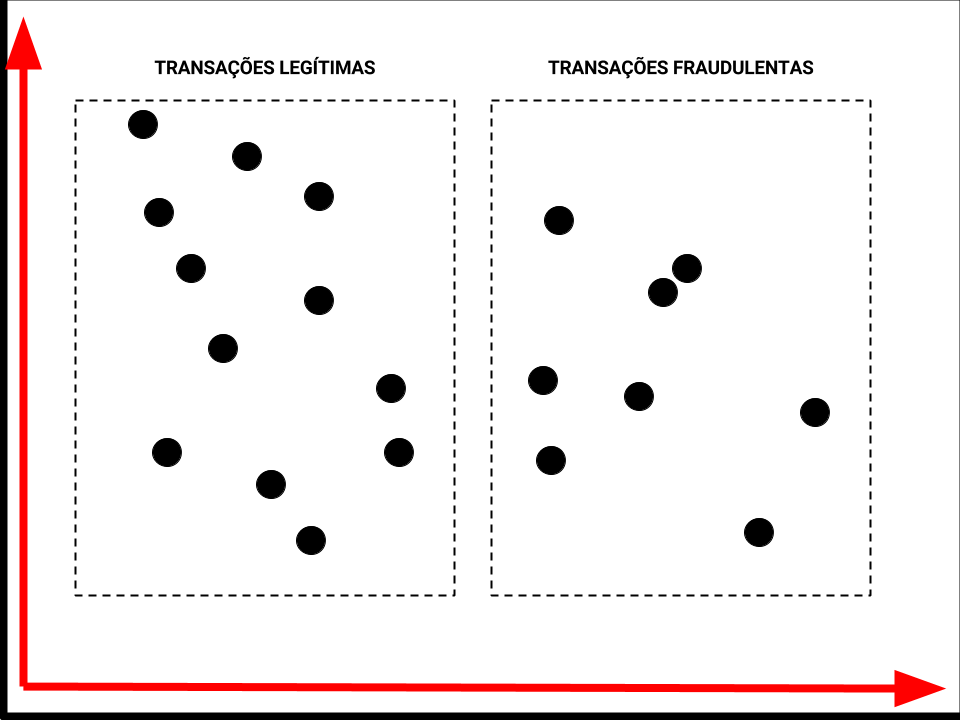
\includegraphics[width=8cm]{figuras/dados-classificados}}
	}{
		\Fonte{Elaborado pelo autor}		
	}	
\end{figure}

Existem alguns algoritmos de classificação muito utilizados como  \textbf{arvore de decisões} e \textbf{Classificação por regras}.


\subsubsection{Classificação com Árvore de decisões}
\label{subsubsec:decision-tree}
Este algoritmo tem com objetivo particionar em classes de forma recursiva os exemplos rotulados, é importante lembrar que este método
utiliza tanto atributos discretos quanto recursivos para classificar. Alguns algoritimos como ID3, ASSISTANT, CART E C4.5 
são utilizados para construção destas árvores de decisão.

Árvores de decisão são facilmente representadas por um fluxograma com a estrutura de uma árvore, onde o ponto de partida é chamado de nó raiz,
além do nó raiz temos os nós terminais e não terminais também conhecidos como ramos e folhas. Posto que os nós não-terminais/ramos se divide em nós filhos,
e está divisão é dada por uma condição sobre o valor de um atributo de um exemplo, enquanto que os nós terminais/folhas não se dividem, ele atribui uma classe ao exemplo.

Dado uma árvore de decisão utilizada para classificar pacientes doentes e saudáveis:

\begin{figure}[ht!]
	\centering
	\Caption{\label{fig:ex-arvore} }	
	\UECEfig{}{
		\fbox{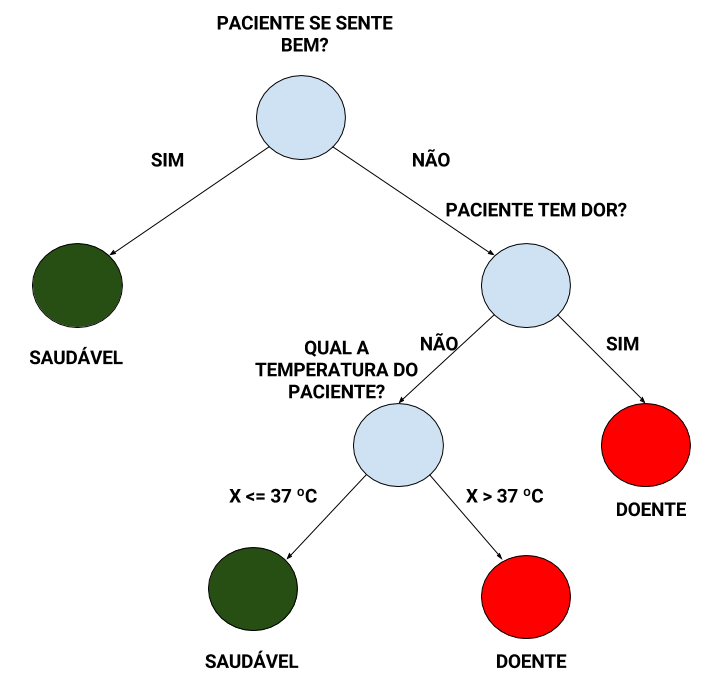
\includegraphics[width=12cm]{figuras/ex-arvore-decisao}}
	}{
		\Fonte{Elaborado pelo autor}		
	}	
\end{figure}

Ao submeter um conjunto de dados de uma paciente com os seguintes atributos {Se sente bem: S, Paciente Sente Dor: N, Temperatura: 38}, 
este exemplo será classificado como doente por conta das regras aplicadas durante o fluxo.

\subsubsection{Regressão}
\label{subsubsec{regressao}}
Regressão assim como em classicação utiliza de exemplos rotulados para treino, porém estes rótulos são baseados em atribudos com valores contínuos, 
diz-se que um atributo é contínuo quando assume qualquer valor numéricos presente em um conjunto infinito em uma determinada escala, por exemplo o preço de uma casa, 
pode ser R\$300.000,00 ou R\$890.092,00. Seu objetivo é identificar um modelo de curva ou uma função linear \textit{y = f(x)}, com base
em parâmetros conhecidos dos exemplos de treino, para prever o valor do \textbf{rótulo} em novos dados.
Por exemplo dado um conjunto de dados de treino que diz respeito à um imóvel, pretende-se identificar um modelo para poder predizer
o preço de imóveis:

\begin{table}[h!]
	\Caption{\label{dados-imoveis} Exemplos rotulado de dados de imóveis}
	\IBGEtab{}{
		\begin{tabular}{rr}
			\toprule
			Área ($m^{2}$) & Preco (R\$) \\
			\midrule \midrule
			192,00  &        250.000,00  \\
			140,55  &        187.000,00  \\
			88,90   &         88.590,00  \\
			73,82   &         69.000,00  \\
			125,50  &        120.456,00  \\
			110,80  &        108.459,00  \\
			400,90  &        800.750,00  \\
			399,90  &        780.000,00  \\
			\bottomrule
		\end{tabular}
	}{
    \Fonte{Produzido pelo autor}
	\Nota{A coluna preço é o rótulo de cada exemplo.}	
}
\end{table} 

Pretende-se identificar um modelo que ao aplicar um novo imóvel com área de \textit{x $m^2$} me retorne o seu possível valor. A figura ~\ref{fig:regressao-plano-cartesiano} ilustra 
o modelo de regressão deste caso, que é basicamente um função linear \textit{y = f(x)}, onde \textbf{\textit{y}} seria o valor que estamos tentando inferir e \textbf{\textit{x}} é o parâmetro 
conhecido que será utilizado, neste caso a área do imóvel.

\begin{figure}[ht!]
	\centering
	\Caption{\label{fig:regressao-plano-cartesiano} }	
	\UECEfig{}{
		\fbox{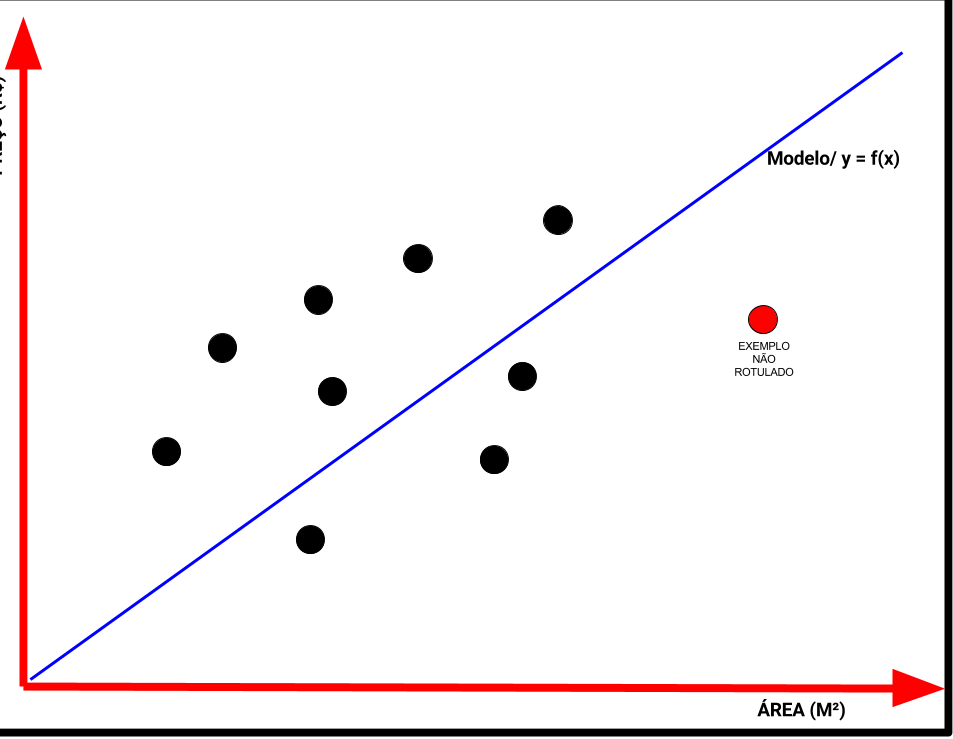
\includegraphics[width=12cm]{figuras/regressao-plano-predicao-imovel}}
	}{
		\Fonte{Elaborado pelo autor}		
	}	
\end{figure}